%%
\documentclass[preprint,12pt]{elsarticle}

\usepackage{amsmath}
%% Use the option review to obtain double line spacing
%% \documentclass[preprint,review,12pt]{elsarticle}

%% Use the options 1p,twocolumn; 3p; 3p,twocolumn; 5p; or 5p,twocolumn
%% for a journal layout:
%% \documentclass[final,1p,times]{elsarticle}
%% \documentclass[final,1p,times,twocolumn]{elsarticle}
%% \documentclass[final,3p,times]{elsarticle}
%% \documentclass[final,3p,times,twocolumn]{elsarticle}
%% \documentclass[final,5p,times]{elsarticle}
%% \documentclass[final,5p,times,twocolumn]{elsarticle}
%\usepackage{feynmp}
\DeclareGraphicsRule{*}{mps}{*}{}
\usepackage[compat=1.1.0]{tikz-feynman}
\providecommand{\LuaTeX}{Lua\TeX}
\providecommand{\tikzfeynmanname}{\tikzname-Feynman}

%% if you use PostScript figures in your article
\usepackage{url}
%% use the graphics package for simple commands


\usepackage{graphics}
%% or use the graphicx package for more complicated commands
\usepackage{graphicx}
%% or use the epsfig package if you prefer to use the old commands
%% \usepackage{epsfig}
%%\usepackage{pifont}%use circled number
\usepackage{booktabs}
\usepackage{longtable}
\usepackage{multirow}
\usepackage{subfig}
%% The amssymb package provides various useful mathematical symbols
\usepackage{amssymb}
%% The amsthm package provides extended theorem environments
%% \usepackage{amsthm}

%% The lineno packages adds line numbers. Start line numbering with
%% \begin{linenumbers}, end it with \end{linenumbers}. Or switch it on
%% for the whole article with \linenumbers after \end{frontmatter}.
%% \usepackage{lineno}

%% natbib.sty is loaded by default. However, natbib options can be
%% provided with \biboptions{...} command. Following options are
%% valid:

%%   round  -  round parentheses are used (default)
%%   square -  square brackets are used   [option]
%%   curly  -  curly braces are used      {option}
%%   angle  -  angle brackets are used    <option>
%%   semicolon  -  multiple citations separated by semi-colon
%%   colon  - same as semicolon, an earlier confusion
%%   comma  -  separated by comma
%%   numbers-  selects numerical citations
%%   super  -  numerical citations as superscripts
%%   sort   -  sorts multiple citations according to order in ref. list
%%   sort&compress   -  like sort, but also compresses numerical citations
%%   compress - compresses without sorting
%%
%% \biboptions{comma,round}

% \biboptions{}


\begin{document}

\begin{frontmatter}

%% Title, authors and addresses

%% use the tnoteref command within \title for footnotes;
%% use the tnotetext command for the associated footnote;
%% use the fnref command within \author or \address for footnotes;
%% use the fntext command for the associated footnote;
%% use the corref command within \author for corresponding author footnotes;
%% use the cortext command for the associated footnote;
%% use the ead command for the email address,
%% and the form \ead[url] for the home page:
%%
%% \title{Title\tnoteref{label1}}
%% \tnotetext[label1]{}
%% \author{Name\corref{cor1}\fnref{label2}}
%% \ead{email address}
%% \ead[url]{home page}
%% \fntext[label2]{}
%% \cortext[cor1]{}
%% \address{Address\fnref{label3}}
%% \fntext[label3]{}

\title{Neutrino Studies and the SNO+ Experiment\\
	Doctoral Candidacy Exam Report
	}

%% use optional labels to link authors explicitly to addresses:
%% \author[label1,label2]{<author name>}
%% \address[label1]{<address>}
%% \address[label2]{<address>}

\author{Jie\quad Hu}

\address{Department of Physics, University of Alberta}

\end{frontmatter}

%%
%% Start line numbering here if you want
%%
% \linenumbers

%% main text
\section{Introduction}

\subsection{Research Backgrounds}
Neutrinos are one type of elementary particles in the Standard Model. The Standard Model is a theory of describing elementary particles and their interactions. It has triumphantly passed various experimental verifications, including the discovery of Higgs bosons in 2012 and has ruled over the field of particle physics for more than 40 years. However, it has been found in experiments that some properties of neutrinos can not be described by the Standard Model, which shows clues of the new physics beyond the Standard Model. This put the studies of neutrinos in the spotlight.

SNO+ is one of the experiments for exploring the unknown properties of neutrinos. Its main research target is to examine the nature of neutrinos: whether they are Majorana or Dirac particles.

\subsection{Early Experiments}
The existence of neutrinos was first proposed by Wolfgang Pauli in 1930s to solve the contradictions observed in beta decay experiments. It was shown definitively by James Chadwick in 1914 that the electrons emitted in beta decay did not have a discrete set of energies but continuous spectrum\cite{cowanexpintro}. This means that the energy, momentum and angular momentum (spin) were not conserved between the nucleus and electron. Pauli introduced a charge-neutral particle with spin 1/2 and a mass scale comparable to electron, then the sum of the energies of neutron and electron is constant, which solved the problem. 

In 1934, Bethe and Peierls suggested direct neutrino detection via a neutrino-induced interaction, the inverse beta decay (IBD): $\bar{\nu}_e\to e^+ + n$. Their calculation showed the IBD cross section of the order of $10^{-43}~cm^2$, which indicates that neutrino is difficult to be detected\cite{bethe1}.
 
However, in 1956, by utilizing a nuclear reactor as an intense neutrino source with neutrino fluxes on the order of $10^{12}-10^{13}$ neutrinos/second/cm$^2$, Fred Reines and Clyde Cowan made a first discovery of the neutrino (specifically, it was electron anti-neutrinos $\nu_e$). Anti-neutrinos from the reactor interacted with the detector tank via IBD. As the tank was filled with water dissolved with cadmium chloride (CdCl$_2$), the produced positrons quickly annihilate with $e^-$ via pair-annihilation and gives $\gamma$ signals while the produced neutrons go through the neutron capture process: 

\noindent$n+^{108}$Cd$\to ^{109}$Cd$^*\to ^{109}$Cd$ +\gamma$ and gives delayed $\gamma$ signals. In addition, the water tank was surrounded by liquid scintillators coupled with photomultiplier tube (PMT) to detect emitted photons. By searching for a coincidence of these two characteristic signals, this provides a distinctive signature for the neutrino reaction. They also measured the cross-section as $6.3\times10^{-44}~cm^2$.

In 1930s, Bethe et al. explained the origin of the Sun's energy comes from a series of subsequent nuclear reactions\cite{bethe2}. In 1964, John Bahcall pointed out that the direct evidence for the existence of nuclear reactions in the interiors of stars can only be proved by the detection of solar neutrinos. Since the endothermic reaction $\nu_e+^{37}$Cl$\to^{37}$Ar$+e^-$ was then the most promising method for solar neutrinos detection, he also predicted the number of absorptions of solar neutrinos by terrestrial $^{37}$Cl atoms\cite{bahcall1}. In the meantime, Raymond Davis designed an experiment that used a 380 m$^3$ tank filled with Perchloroethylene (C$_2$Cl$_4$), a dry-cleaning fluid rich in chlorine. Solar neutrinos are expected to change $^{37}$C1 to $^{37}$Ar and the produced $^{37}$Ar were extracted and counted. The energy threshold ($E_{thresh}$) of the experiment is 0.814 MeV, which gives a measurement of $^8$B neutrino fluxes\cite{raymond}. Their first results announced in 1968 showed that only about one third of radioactive argon atoms were measured compared to the prediction, which soon raised a problem of missing solar neutrinos. 

Later in 1990s, GALLEX and SAGE operated for lower energy solar neutrino detection via gallium reaction: $\nu_e+^{71}$Ga$\to^{71}$Ge$+e^-$, with an $E_{thresh}$ = 233.2 keV. This low threshold enables the gallium experiments to detect pp neutrinos, which constitute about 90\% of the neutrinos predicted by standard solar models. The results of the gallium experiments further confirmed the discrepancies as well as provided fundamental constraints on solar models\cite{GALLEX,SAGE,bahcall2}.

Cosmic rays from outer space continuously interaction with nuclei in the atmosphere and produce secondary particles. Atmospheric neutrinos come from decay products of the hadrons in the secondaries. The dominate processes of atmospheric $\nu_e$ and $\nu_\mu$ production is $\pi^+\to\mu^+ + \nu_\mu$ followed by $\mu^+ \to e^+ + \bar{\nu}_\mu + \nu_e$. In 1980s, Kamiokande in Japan was one of the experiments that were able to measure atmospheric neutrinos. They used a 3-kton water-Cherenkov detector to count the Cherenkov rings caused by neutrino charged current interactions in the detector. The $\nu_e$ interaction produces electron that produces elect
ro-magnetic shower during its propagation in the water while the $\nu_\mu$ interaction produces muon that propagates almost straightly without producing electro-magnetic shower. Then $\nu_\mu$ ($\mu$-like events) are separated from $\nu_e$ ($e$-like events) by the fact that $\mu$-like events create sharper Cherenkov rings. Kamiokande measured the ratio of fluxes $\Phi(\nu_\mu+\bar{\nu}_\mu)/\Phi(\nu_e+\bar{\nu}_e)$. The fluxes of atmospheric neutrinos are well understood and the ratio $\nu_\nu/\nu_e$ is expected to be $\sim$2 at low energies $\leq$1~GeV. In 1988, they found a deficit of measured $\mu$-like events compared to the prediction, which was later confirmed by IMB in 1992\cite{imb} and Soudan-2 in 1997\cite{soudan2} and called ``atmospheric neutrino anomaly''\cite{atmNuReview}. At the meantime, by the ability to detect directional information of particles, they were able to observe the solar neutrinos by checking whether neutrinos were pointing away from sun. They also found that only about 1/2 of $^8$B solar neutrino flux was measured compared to the solar models\cite{kamioII}. 

\section{Neutrino Flavor Mixing}
\subsection{The SNO and Super-K Experiment}
The facts of solar neutrino missing and loss of atmospheric neutrinos indicate that a neutrino can change its flavor or oscillate during propagation.

To resolve the solar neutrino problem with a direct approach, Herbert Chen in 1984 proposed an experiment using a large heavy water (D$_2$O) Cherenkov detector to distinguish the flavors of solar neutrinos\cite{herbertChen}. This proposal later lead to the SNO collaboration. The neutrino disintegration of the deuteron ($d$) is expected and the SNO detector is sensitive to solar neutrinos from $^8$B decay via three interactions: (1) the charged current (CC): $\nu_e+d\to e^-+p+p$ , (2) the neutral current (NC): $\nu_x+d\to\nu+p+n$, (3) the elastic scattering (ES): $\nu_x+e^-\to \nu_x+e^-$. The CC channel is only sensitive to $\nu_e$ while the NC is independent of the neutrino type, which can provide a total measurement of solar neutrino flux even if neutrinos change flavor. The ES channel is also sensitive to all flavors but with reduced sensitivities to $\nu_\mu$ and $\nu_\tau$\cite{SNO}.

In 2002, SNO reported that the measured total $^8$B solar neutrino flux ($\Phi_{NC}$) is consistent with solar models while the $\nu_e$ component of the flux ($\Phi_e$) is about 1/3 of the $\Phi_{NC}$\cite{SNO}:
\[
P_{SNO} = \frac{\Phi_e}{\Phi_{NC}}= 0.340\pm0.023^{+0.029}_{-0.031}
\]

These results indicate that about 2/3 of the original solar $\nu_e$ have transformed to $\nu_{\mu,\tau}$ when they arrived the earth. This explains the problem of missing solar neutrinos. The final results of SNO published in 2013\cite{SNOresult} for $^8$B neutrino flux are:
\[
\Phi_{total} = \sum_{f=e,\mu,\tau}\Phi(\nu_f)= 5.25\pm0.16(stat.)_{-0.13}^{+0.11}(sys.)\times10^6~cm^{-2}s^{-1}
\]
\[\Phi(\nu_\mu)+\Phi(\nu_\tau)=(3.26\pm0.25^{+0.40}_{-0.35})\times 10^6~cm^{-2}s^{-1}
\]

In 1996, the Kamiokande experiment was upgraded to Super-Kamiokande (Super-K) with a 50-kton water Cherenkov detector. In two years, Super-K measured sufficient atmospheric neutrinos and announced a striking discovery: the number of high energy muon neutrinos is zenith angle dependent and caused a deficit of up-going $\nu_\mu$. 

The measured up-going muon neutrinos are mostly created in the atmosphere at the opposite side of the Earth to the Super-K detector and travel about 12800 km while the downward-going muon neutrinos are created in the atmosphere about 15 km above the detector. The measured $\nu_e$ in the same scenario do not show such deficit.

Therefore, a natural explanation for the results is that the up-going muon neutrinos have oscillated to $\nu_\tau$ during their thousands of kilometres travel. The Super-K results are consistent with two-flavor $\nu_\mu\leftrightarrow\nu_\tau$ oscillations\cite{superK}.

\subsection{Theory}
Both SNO and Super-K discovered the phenomenon of neutrino flavor conversions directly and were awarded the 2015 Nobel Prize. The phenomenon suggests that neutrino has a small but finite mass and a violation of lepton number conservation, which is not expected in the Standard Model. Actually, as early as 1957, Pontecorvo had already suggested an oscillation of $\nu\leftrightarrow\bar{\nu}$, and later worked out a phenomenological model for $\nu_e\leftrightarrow\nu_\mu$ in theory\cite{nobeldoc}. Maki, Nakagawa and Sakata further 

small differences between the masses of the three neutrino states, as well as an
inequivalence between neutrino flavor and mass eigenstates.


The flavor of a neutrino is determined as a superposition of the mass eigenstates.

for two-neutrino oscillation, 

\[
\begin{bmatrix}
\nu_e\\
\nu_\mu\\
\end{bmatrix}
= \begin{bmatrix}
\cos\theta_{12} &\sin\theta_{12}\\
-\sin\theta_{12} &\cos\theta_{12}\\
\end{bmatrix}
\begin{bmatrix}
\nu_1\\
\nu_2\\
\end{bmatrix}
\]

\[
|\nu_e> = \exp\{-iE_1t\}\cos\theta_{12}|\nu_1>+\exp\{-iE_2t\}\sin\theta_{12}|\nu_2>
\]

for ultra-relativistic neutrinos, the momentum $|\vec{p}|=p\simeq E>>m$, then $E_1\simeq p+\frac{m_1}{2p}$ and $E_2\simeq p+\frac{m_2}{2p}$



Oscillations of neutrinos are caused by flavor of lepton mixing in vacuum.

Neutrino oscillations and flavor conversions are caused by mixing.

\[
|\nu_f> = \sum_{k=1}^3U^*_{fk}|\nu_k> 
\]
where $f=e,\mu,\tau$ and $k=1,2,3$
%%nu oscillation matrix
%\[
%\begin{bmatrix}
%\nu_e \\
%\nu_\mu  \\
%\nu_\tau  \\
%\end{bmatrix}
%= U
%\begin{bmatrix}
%\nu_1 \\
%\nu_2  \\
%\nu_3  \\
%\end{bmatrix}
%\]

The hermite matrix U is the PMNS matrix and can be parametrized as
\[
U=
\begin{bmatrix}
1 &0 &0\\
0 &\cos\theta_{23} &\sin\theta_{23}\\
0 &-\sin\theta_{23} &\cos\theta_{23}\\ 
\end{bmatrix}
\begin{bmatrix}
\cos\theta_{13} &0 &e^{-i\delta_{CP}}\sin\theta_{13}\\
0 &1 &0\\
e^{-i\delta_{CP}}\sin\theta_{13} &0 &\cos\theta_{13}\\ 
\end{bmatrix}
\begin{bmatrix}
\cos\theta_{12} &\sin\theta_{12} &0\\
-\sin\theta_{12} &\cos\theta_{12} &0\\
0 &0 &1\\ 
\end{bmatrix}
\]

In PMNS matrix, we have four parameters:
$\theta_{13}$ for reactor neutrino and accelerator
$\delta_{CP}$ for CP violation, $\theta_{23}$ is atmospheric neutrino , $\theta_{12}$ for solar neutrino. 


two mass difference squares, $\Delta m^2_{12}=m_1^2-m_2^2$ and $\Delta m^2_{23}=m_2^2-m_3^2$
totally six parameters, .

oscillation in vacuum

two-generation neutrino model

For a neutrino with energy $E_\nu$, after flying for a distance of $L$, the oscillation probability is: 
\[
P(\nu_e\to\nu_{\nu})=\sin^2(2\theta)\sin^2\Big(\frac{1.27\Delta m^2(eV^2)L(km)}{E_\nu(GeV)}\Big)
\]



to determine the regions of , 


neutrino energy scale, 
$\theta_{12}$ is mainly measured by solar and reactor experiments, while $\theta_{12}$ is measured by atmospheric and accelerator experiments. 






Compared to solar and atmospheric neutrino experiments, reactor antineutrino experiments have 
less uncertainties in the rate and energy spectrum of incoming $\bar{\nu}_e$s.
  
In 2003, the Kamioka Liquid Scintillator Anti-Neutrino Detector (KamLand) discovered the reactor $\bar{\nu}_e$ ($E_{\bar{\nu}_e}>3.4$ MeV) disappearance over a long base of 180 km at 99.95\% C.L.. 
If CPT invariance is assumed, 
ruled out except the LMA solution\cite{kamland}.
L/E dependence 
$\Delta m_{12}^2$ and $\theta_{12}$
LMA MSW solution.

Combined with solar neutrino data, their more precise measurements obtained $\Delta m^2_{12} = 7.59^{+0.21}_{-0.21}\times 10^{-5}eV^2$ and $\tan^2{\theta}_{12}=0.47^{+0.06}_{-0.05}$\cite{kamland_measure}.





The third mixing angle $\theta_{13}$ is mainly searched by the experiments designed for reactor $\bar{\nu}_e$ disappearance over baselines of $\sim$1 km. In late 1990s, CHOOZ and Parlo Verde experiments set an upper limit of $\sin^2 2\theta_{13}<0.12$ at 90\% C.L.\cite{joseTextbook}.

Three experiments, Double CHOOZ, DayaBay and RENO 

In 2011, the Daya Bay Experiment was built and is able to measure $\theta_{13}$ with a sensitivity of $\sin^2 2\theta_{13}\sim 0.01$.
In 2012, Daya Bay reported the discovery of non-zero $\theta_{13}$ with a significance of 5.2$\sigma$, which was confirmed by RENO and Double Chooz experiments in the same year. A more recent value from Daya Bay is reported in 2016\cite{dayabayresults}, based on 1230 days of operation and $\bar{\nu}_e$ data from eight detectors, $\sin^2 2\theta_{13} = 0.0841\pm0.0027(stat.)\pm0.0019(syst.)$. This high-precision result makes $\sin^2 2\theta_{13}$ the best measured mixing angle\cite{reactorNu}. 

From these measured results, it is obvious to conculde that the mixing angles between neutrinos are very different to the quark mixing angles. 




\subsection{Matter Effects}
The SNO results, $P_{SNO}$, can not be explained by the neutrino oscillation only, but together with the matter effects, also called Mikheyev-Smirnov-Wolfenstein (MSW) mechanism. The mechanism is caused by the electron neutrinos interact with ambient electrons and nucleons in matter such as the Sun, the Earth.

coherent forward elastic scattering.


In addition to the $H_0$,   
resonant enhancement.



When $\nu_e$ travel through the Sun from the centre to the surface, they interact with the electrons in the Sun. The electron number density $N_e$ in the Sun decreases approximately following the equation: 
\[
N_e(x)=N_e(x_0)\exp\{-\frac{x-x_0}{r_0}\}
\]
where $x-x_0\simeq d$ is the distance $\nu_e$ travelled in the Sun, $x_0$ is the point where solar $\nu_e$ produced in the Sun and $r_0\sim 0.1R_{\odot}$ 

\cite{pdg2017}


The ratio of the matter effects to the vacuum effects is given by: 
\[
R=\frac{2\sqrt2 G_Fn_eE_\nu}{\Delta m_{12}^2}
\]


the large mixing angle (LMA) realization of the MSW mechanism.


\subsection{Solar Neutrino}

two sets of fusion reactions 

solar $\nu_e$ produced and propagate from the centre of the Sun to the Sun surface.  



CNO(carbon–nitrogen–oxygen) cycle
pp chain(proton–proton chain reaction)

pp chain is dominant in 

neutrino mass


Solar Neutrinos

The Borexino experiment later detected the $^7$Be neutrinos and CNO neutrinos at $\sigma$.


Among the three interactions, (1) is only for $\nu_e$; (2) and (3) are for all types of neutrinos. In addition, in (3), the $\nu_e$ is expected to be than the other types.  

The third phase of the SNO experiment,  gave a 



 experiment: early exp:   Tritron decay measurements , put limits on mass
 
 for Dirac neutrinos, the origin of the neutrinos mass is the same Higgs mechanism while a right-handed component of the neutrino fields must be introduced into SM. This helps to eliminate the asymmetry in the standard model.  Call minimally extended SM.
 
 right-handed field is sterile. do not participate in weak interactions, strong and EM. only gravitational.
 normal left-handed ->weak, call active
 
 number of right-handed fields is not constrained. for 3 generation, introducing 3 right-handed fields is not even an extension of SM.


\section{Double Beta Decay}


double beta decay ($2\nu\beta\beta$)
$(Z,A) \to (Z+2,A)+2e^{-}+2\bar{\nu_e}$


Neutrinoless double beta decay, 
$0\nu\beta\beta$

In 1937, Ettore Majorana  
Majorana fermion that is its own antiparticle. 


\begin{tikzpicture}
\begin{feynman}
\vertex (a1) {\(d\)};
\vertex[right=1.5cm of a1] (a2);%% W- goes out

\vertex[above=2em of a2] (vv1);\vertex[right=1cm of vv1] (v1);
\vertex[right=1cm of v1] (v3){\(e^{-}\)};
\vertex[above=4em of a2] (vv2);\vertex[right=1cm of vv2] (v2);
\vertex[right=1cm of v2] (v4){\(e^{-}\)};


\vertex[right=2cm of a2] (a3) {\(u\)};
\vertex[below=1em of a1] (b1) {\(d\)};
\vertex[below=1em of b1] (b2) {\(u\)};
%top n
\vertex[above=6em of a1] (aa1) {\(d\)};\vertex[right=1.5cm of aa1] (aa1v);%%W- goes out
\vertex[above=1em of aa1] (aa2) {\(d\)};
\vertex[above=1em of aa2] (aa3) {\(u\)};

%% Equivalent way to obtain (d):
%%top right p = udu
\vertex[above=6em of a3] (c1) {\(u\)};
\vertex[above=1em of c1] (c2) {\(d\)};
\vertex[above=1em of c2] (c3) {\(u\)};
%%bottom right p = udu
\vertex[below=1em of a3] (d1) {\(u\)};
\vertex[below=1em of d1] (d2) {\(d\)};

\diagram* {
	(a1) -- [fermion] (a2) -- [fermion] (a3),
	(b1) -- [fermion] (d1), 
	(b2) -- [fermion] (d2), 
	(aa1) -- [fermion] (aa1v) -- [fermion](c1),
	(aa2) -- [fermion] (c2),
	(aa3) -- [fermion] (c3),

	(a2) -- [boson,edge label=\(W^{-}\)] (v1),
	(v2) -- [boson,edge label=\(W^{-}\)] (aa1v),
 
	(v1) -- [fermion] (v3)
    (v2) -- [fermion] (v4)
    (v1) -- [plain] (v2)
	
};
\draw [decoration={brace}, decorate] (b2.south west) -- (a1.north west)
node [pos=0.5, left] {\(n\)};
\draw [decoration={brace}, decorate] (aa1.south west) -- (aa3.north west)
node [pos=0.5, left] {\(n\)};
\draw [decoration={brace}, decorate] (c3.north east) -- (c1.south east)
node [pos=0.5, right] {\(p\)};
\draw [decoration={brace}, decorate] (a3.north east) -- (d2.south east)
node [pos=0.5, right] {\(p\)};
\end{feynman}
\end{tikzpicture}


The most sensitive probe for Majorana neutrinos is a nuclear process
known as neutrinoless double $\beta$ decay ($0\nu\beta\beta$)

\section{Current and Prospect Neutrino Experiments}
Diverse technologies for the neutrino detection have been developed during the past decades. 
\subsection{Solar Neutrino Experiments}

Borexino


\subsection{Reactor Neutrino Experiments}



\subsection{Atmospheric Neutrino Experiments}

ANTARES

IceCube 

DUNE

\subsection{Neutrinoless Double Beta Decay Experiments}
yield information on the absolute neutrino mass scale.
$^{76}$Ge, $^{136}$Xe, $^{130}$Te

The GERmanium Detector Array (GERDA) experiment searches for $0\nu\beta\beta$ of $^{76}$Ge. The experiment uses bare germanium crystals with an enrichment of up to $\sim$87\% $^{76}$Ge operated in a radiopure cryogenic liquid argon (LAr). GERDA Phase I had an exposure of 21.6 kg$\cdot$yr and Phase-II started with 35.6kg from enriched material in December 2015. With combined data of Phase I and Phase II, GERDA reported in 2016 a lower limit half-life of $T^{0\nu}_{1/2}(^{76}$Ge$)>5.3\times 10^{25}$ years at 90\% C.L.\cite{gerda,gerda2}.

The Enriched Xenon Observatory (EXO) experiment uses 200-kg liquid Xenon (LXe) time projection chamber (TPC) to search for $0\nu\beta\beta$ in $^{136}$Xe. In 2011 they observed the half life of double beta decay of $^{136}$Xe to be $2.11\times 10^{21}$ years and in 2014 they set a limit on $T^{0\nu}_{1/2}(^{136}$Xe$)>1.1\times 10^{25}$ yr\cite{exo}. EXO is now upgrading to the next 5-tonne experiment (nEXO) and is expected to reach an exclusion sensitivity of $T^{0\nu}_{1/2}(^{136}$Xe) to about $10^{28}$ years at 90\% C.L.\cite{nEXO}.

Also looking into $^{136}$Xe, the KamLAND-Zen experiment exploits the existing facilities of KamLAND by setting a 3.08-m-diameter spherical inner balloon filled with 13 tons of Xe-loaded liquid scintillator at the center of the KamLAND detector. Their 2016 results from a 504 kg$\cdot$yr exposure obtained a lower limit for the $0\nu\beta\beta$ decay half-life of $T^{0\nu}_{1/2}(^{136}$Xe$)>1.07\times 10^{26}$ yr at 90\% C.L. and the corresponding upper limits on the effective Majorana neutrino mass are in the range 61-165 meV\cite{kamlandZen}.

The Cryogenic Underground Observatory for Rare Events (CUORE) experiment searches for $0\nu\beta\beta$ in $^{130}$Te. CUORE is a ton-scale cryogenic bolometer array that arranges 988 tellurium dioxide (TeO$_2$) crystals. CUORE reported first results in 2017 after a total TeO$_2$ exposure of 86.3 kg$\cdot$yr. Combined with their early data, they placed a lower limit of $T^{0\nu}_{1/2}(^{130}$Te$)>1.5\times 10^{25}$ yr at 90\% C.L. and $m_{\beta\beta}<(140-400)$  meV\cite{cuore}.

\section{SNO+ Experiment}
\subsection{Physics Purpose}
The SNO+ experiment is the successor of the SNO experiment, which makes use of the SNO detector structure, consisting of an acrylic vessel (AV) sphere of 6-m in radius and 5.5-cm in thickness. The detector is placed in a rock cavity filled with .  

a depth of 6000 meter water equivalent (m.w.e)

The main effort taken for the upgrading is to switch the detector medium from heavy water to the scintillator, which has a higher light gain and lowers the detector threshold. 

\cite{whitepaper}

The SNO+ detector is designed for multi-purpose measurements of the neutrino physics.
The experiment will go through three phases: 

1. The water phase: 
Phase-I, the detector will be filled with about 7000 tonnes of ultra-pure water ;

2. The
In the final phase, natural Tellurium will be loaded into the scintillator, in which $^{130}$Te as the source of double beta decay isotope.
Meanwhile, 


\section{The Projects in SNO+}
\subsection{Wavelength Shifter (WLS) Study}
There was a proposal of adding the wavelength shifter (WLS) into the SNO+ detector during the water phase. The specific wavelength shifter we considered is the 2,5-Diphenyloxazole (PPO), which will also be used in the SNO+ scintillator phase and te-loaded phase. Although the proposal will not happen for SNO+ due to the experiment schedule, it is still worthwhile for studying a SNO+-like detector which uses water-based wavelength shifter (water-WLS) as medium.

The advantage of water-WLS detector is to increase the light yield while still keeps the directionality. the PMT distributions of 

Fig.~\ref{PMT_5MeV_water}

Although there are much more isotropic lights, the Cherenkov ring still can be seen clearly, which indicates the .

\begin{figure}[htbp]
	\centering	
	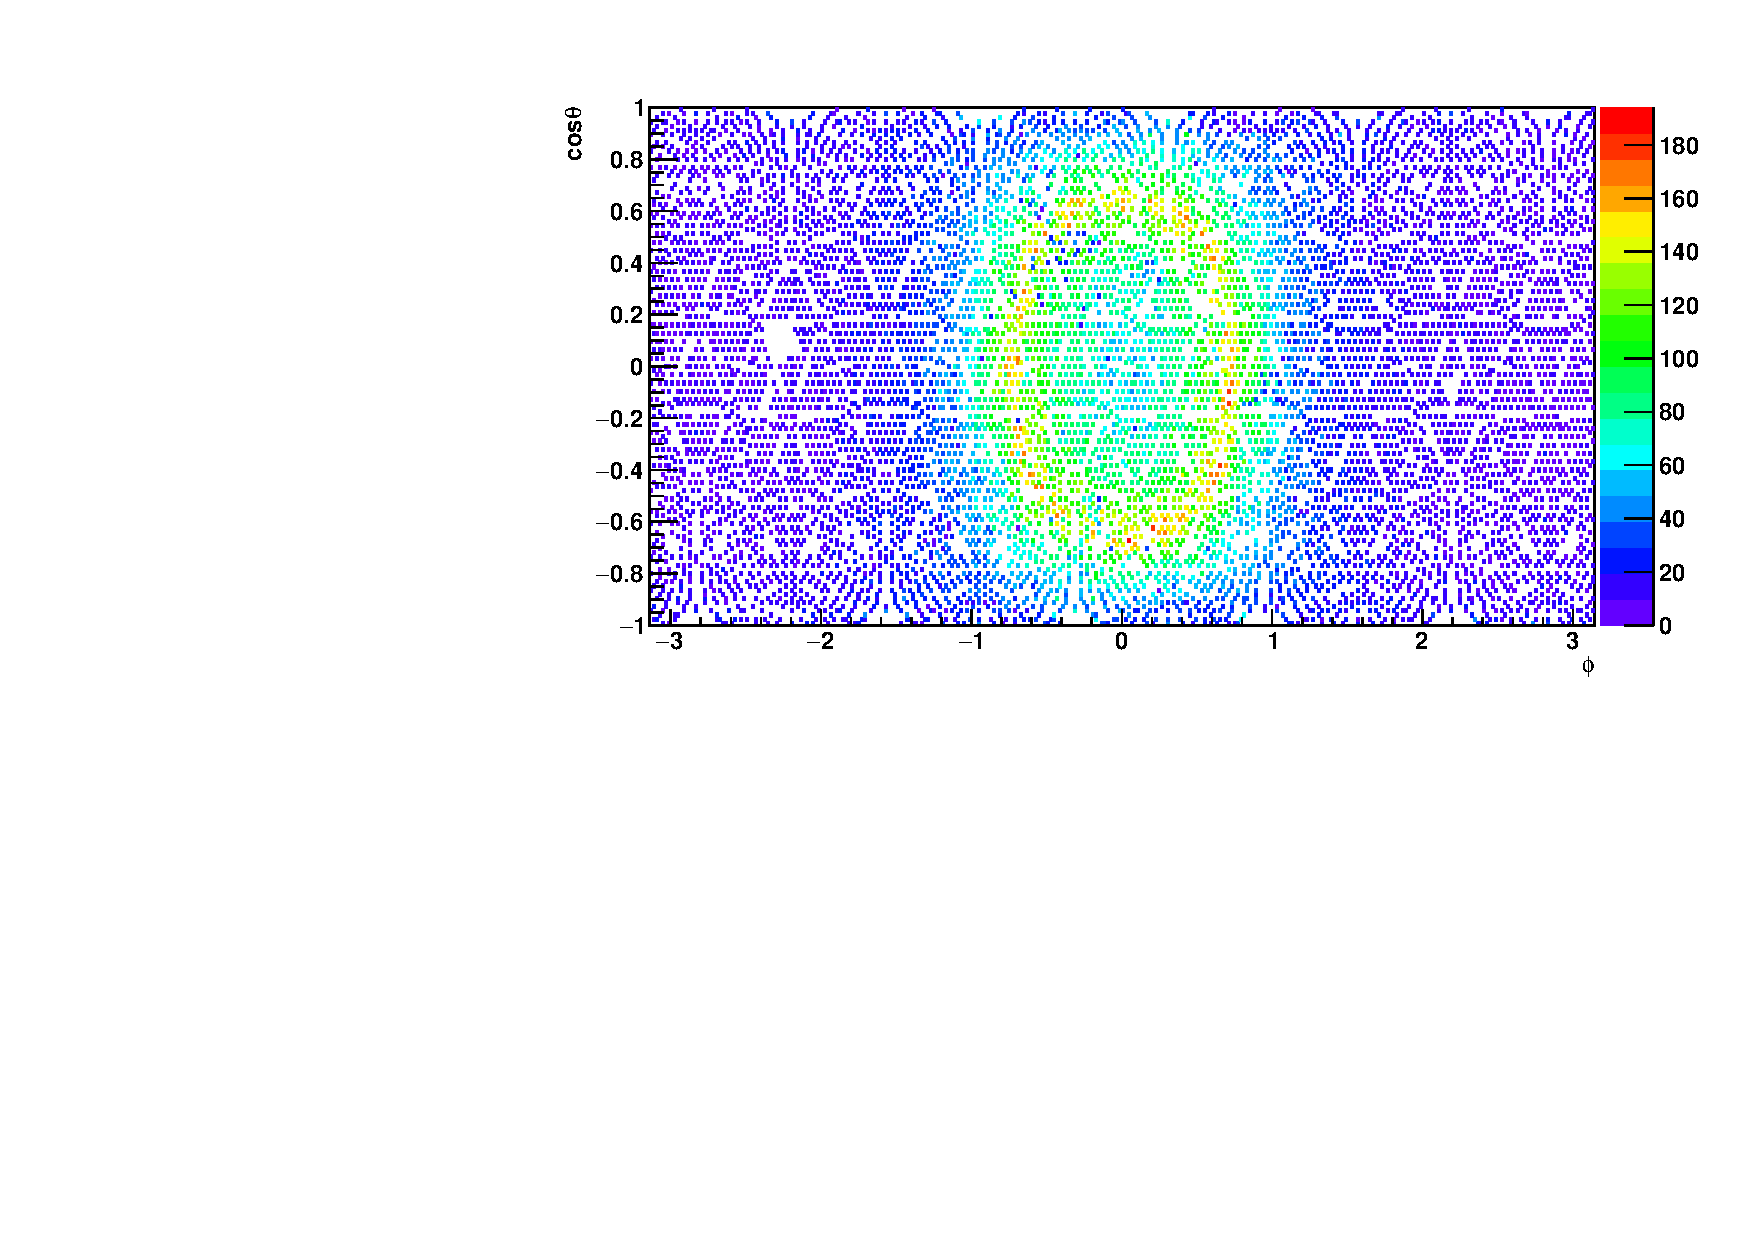
\includegraphics[width=6cm]{PMT_5MeVElectronWater.pdf}
	\caption{\label{PMT_5MeV_water} 
		Distributions of PMT hit for 5 MeV $e^-$ travelling along +x direction in water.
	}
\end{figure}

\begin{figure}[htbp]
	\centering	
	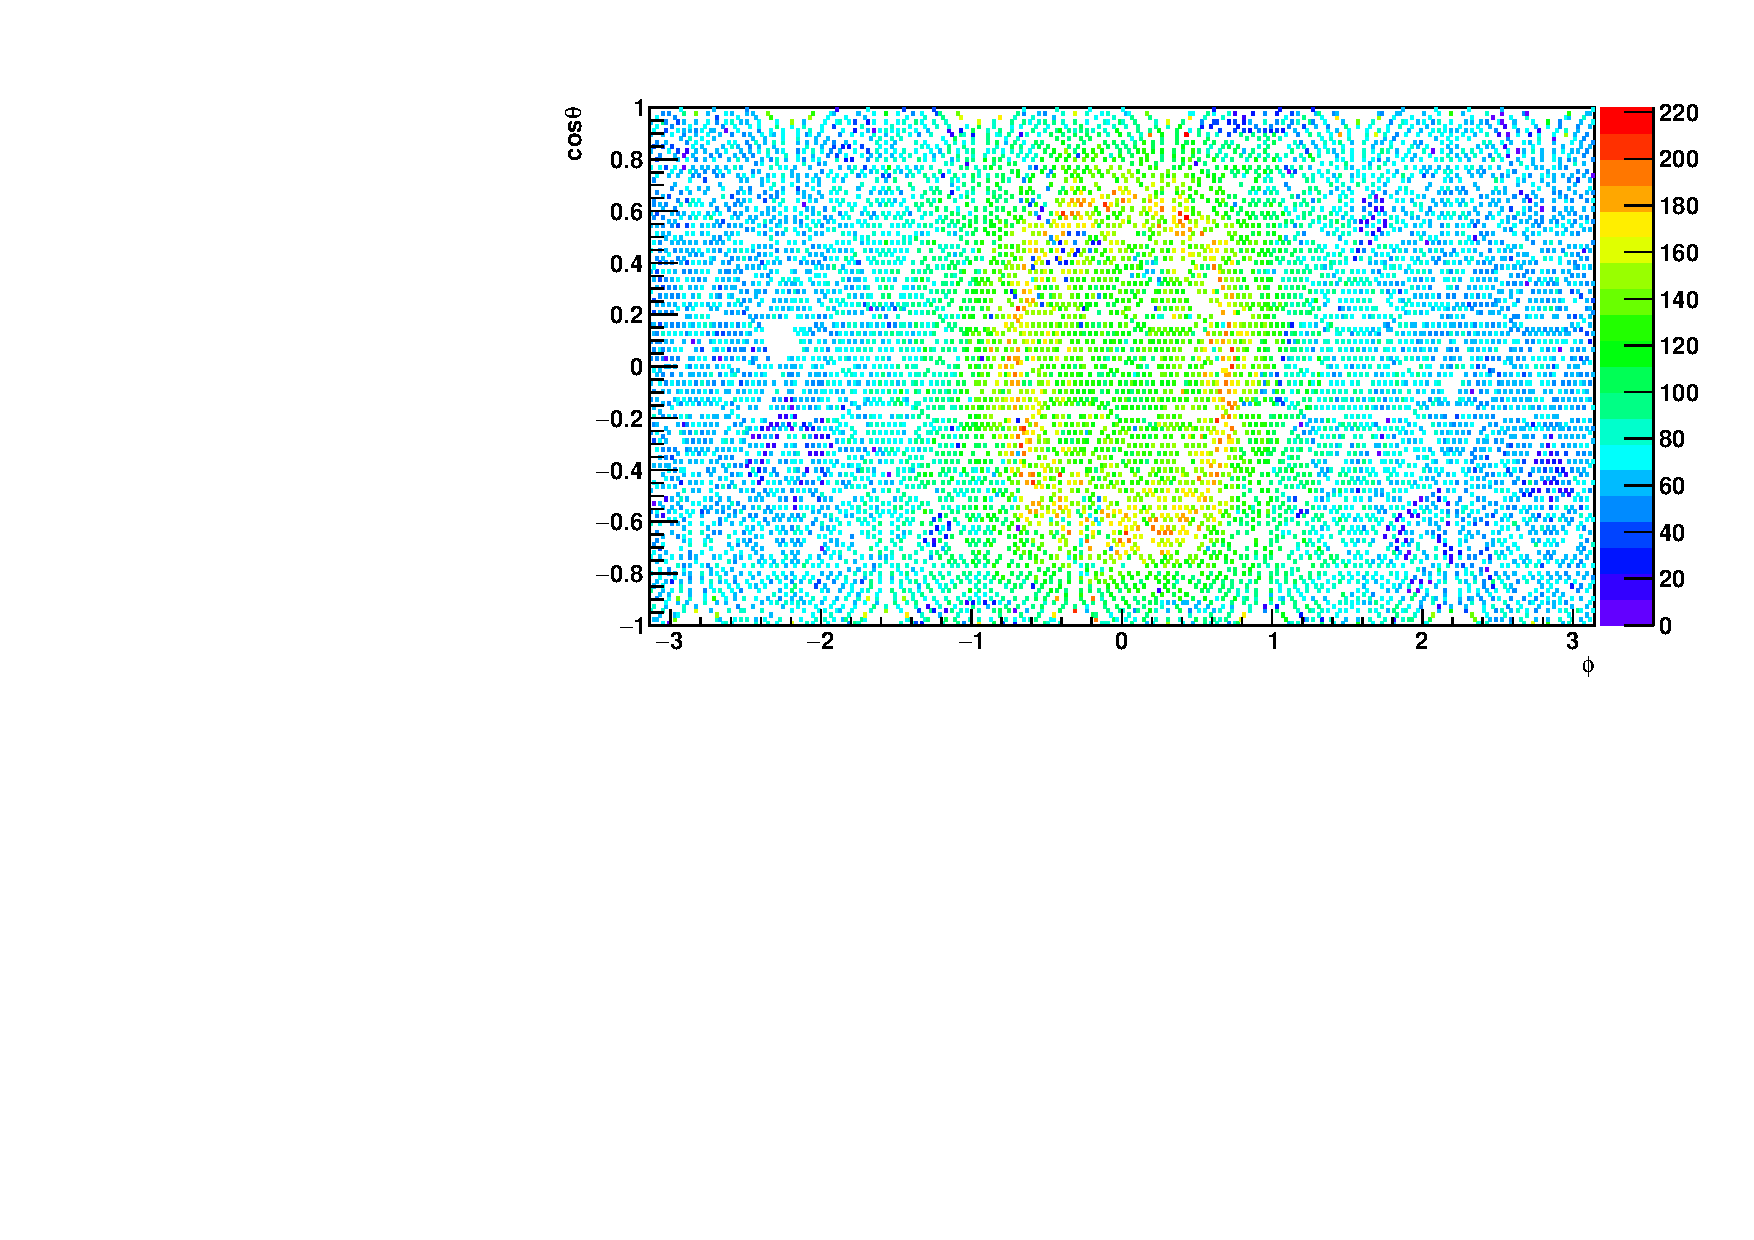
\includegraphics[width=6cm]{PMT_5MeVElectron0p1ppmPPO.pdf}
	\caption{\label{PMT_5MeV_0p1ppmPPO} 
	Distributions of PMT hit for 5 MeV $e^-$ travelling along +x direction in water plus 0.1 ppm PPO.
	}
\end{figure}



In Fig.~\ref{FitterDiagram}, an event is generated at a vertex, travelling along the momentum direction and emits prompt lights. These lights are probably absorbed by the wavelength shifter and then re-emitted at a shifted vertex which along the same direction of the particle momentum. Then $\overrightarrow{shifted~vertex}=\overrightarrow{vertex}+offset\cdot \vec{n}$.  
The offset we set in the fitter is 100 (mm) from the fitter optimization tests. 

\begin{figure}[htbp]
	\centering	
	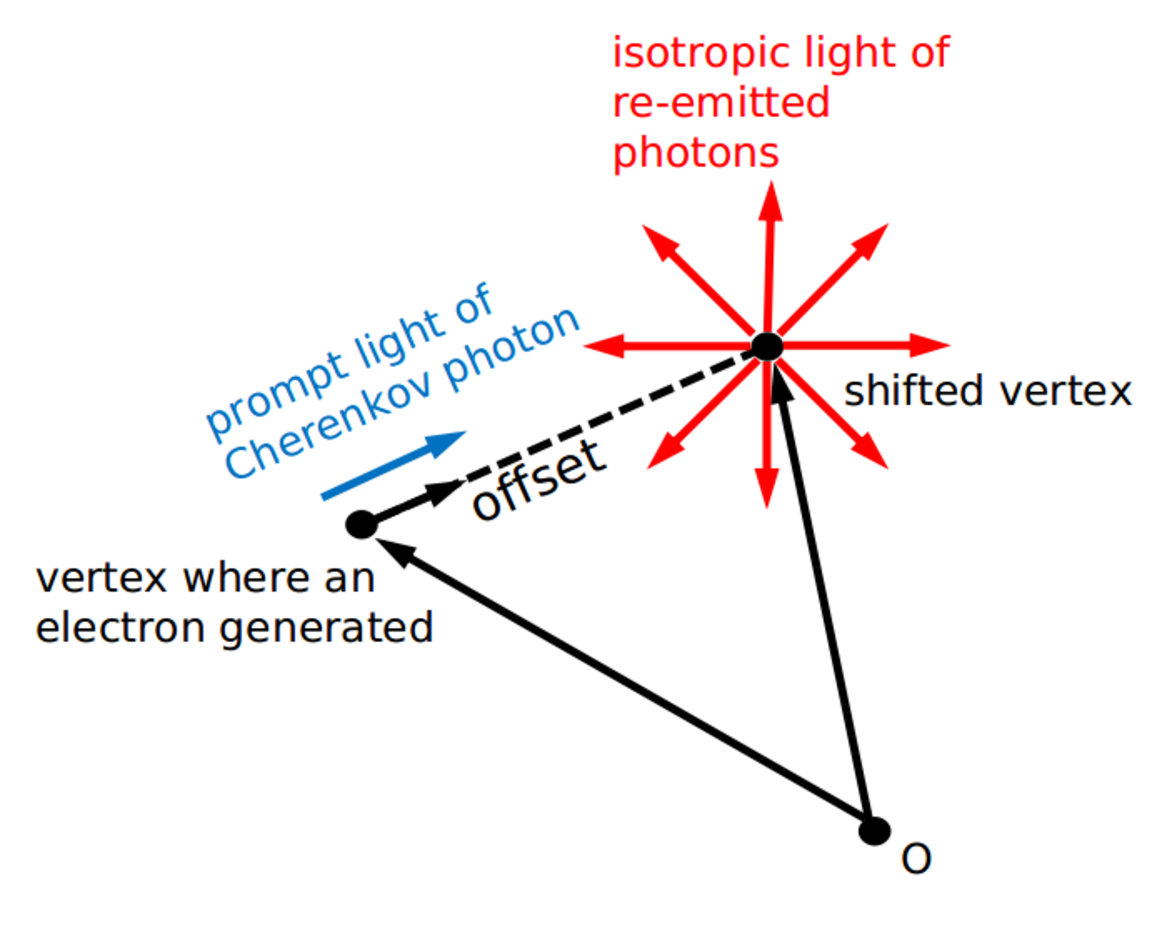
\includegraphics[width=6cm]{FitterDiagram.pdf}
	\caption{\label{FitterDiagram} 
		A diagram shows the fitter geometry.
	}
\end{figure}

\section{Multi-Path Fitter Development}

The Multi-path Fitter (MPW) is an alternative fitter developed for SNO+. It fits for position, time and direction of an event.

- PMT response time (timing) pdf for the position reconstruction, as shown in \ref{MPW_timingPDF}. It is the measured PMT response time distribution from SNO time and the late light response is forced to be de-weighted.

\begin{figure}[!htb]
	\centering
	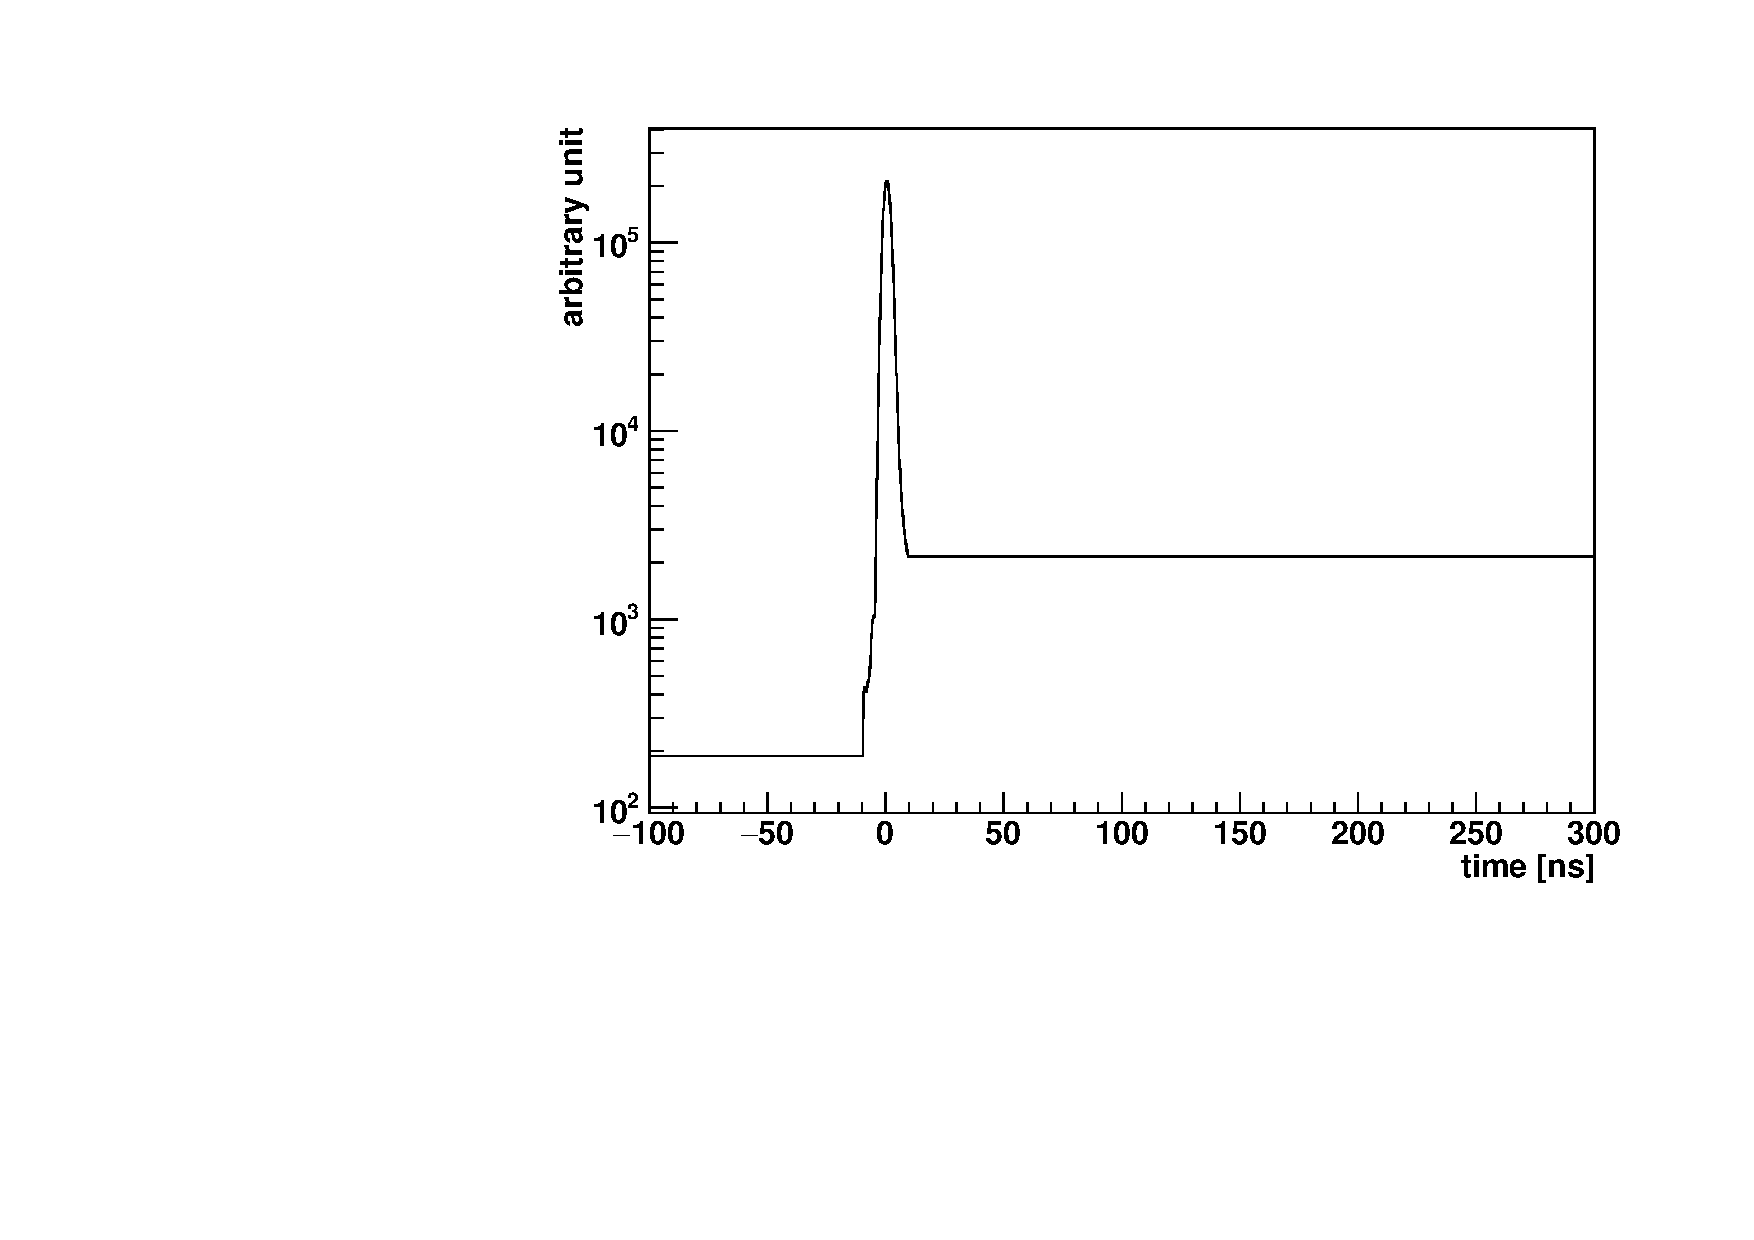
\includegraphics[width=6cm]{MPW_timingPDF.pdf}
	\caption{PMT response time as the timing pdf.}
	\label{MPW_timingPDF}
\end{figure}

- PMT angular response pdf for the direction reconstruction, as shown in \ref{MPW_angularPDF}. It is taken from the Monte Carlo simulation of 5 MeV electrons traverse in the AV with one direction.

\begin{figure}[!htb]
	\centering
	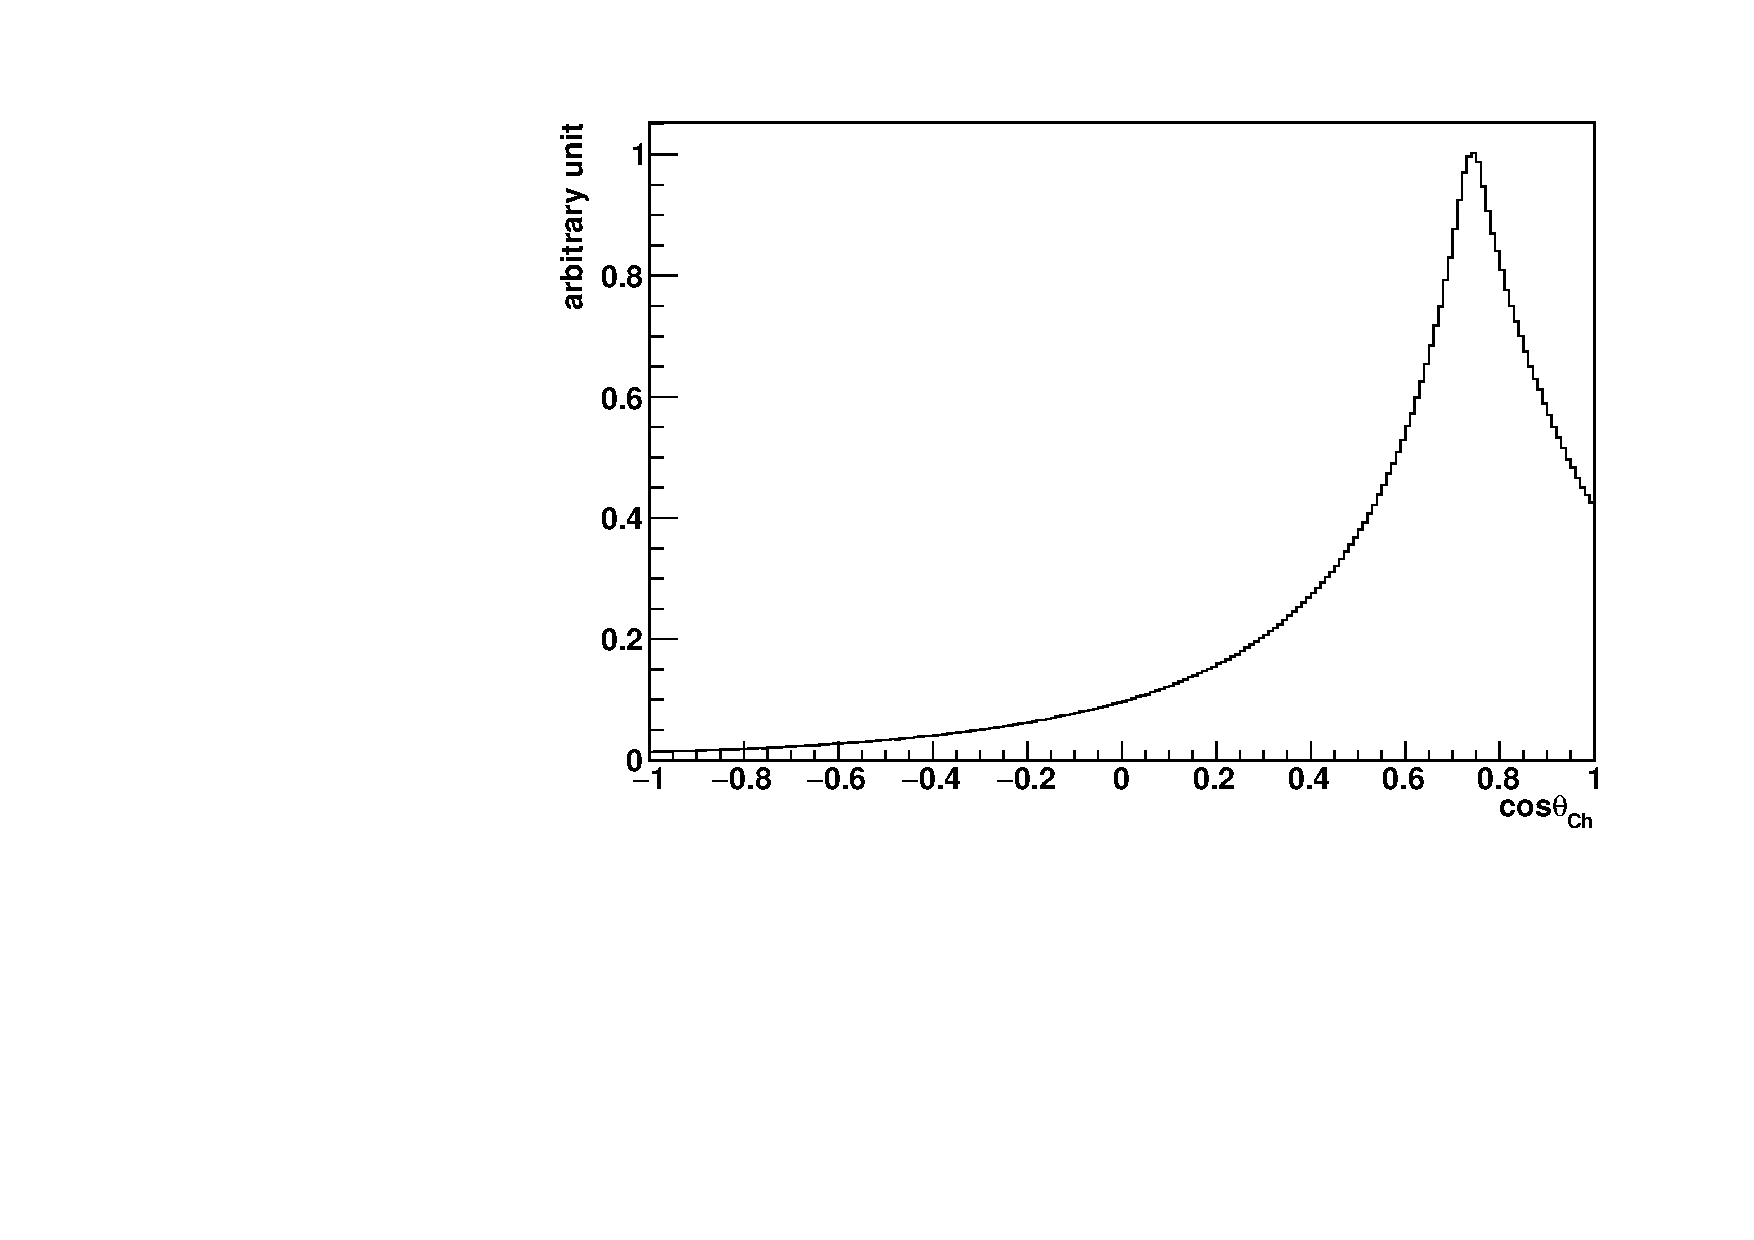
\includegraphics[width=6cm]{MPW_angularPDF.pdf}
	\caption{PMT angular distribution as the angular response pdf.}
	\label{MPW_angularPDF}
\end{figure}

The fitter uses prompt light and straight line paths for likelihood calculations. Then it utilizes the Multi-path Fitter to maximize the likelihood functions and find the best-fit values. The concept of this fitter is the same of the QSNO fitter in SNO time.


\section{$^{16}$N Calibration to SNO+}
The SNO+ detector is currently filled with water and has been under water phase operation for almost a year. In order to calibrate the detector, an $^{16}$N calibration source inherited from the SNO experiment was deployed for Z-axis scan runs in June and full axis scans in November, 2017. 

I apply the current SNO+ reconstruction methods to old SNO $^{16}$N calibration data and the corresponding Monte Carlo simulations to check the position and direction resolutions of the SNO+ algorithms. The results are comparable to those from SNO. A SNO+ energy response processor is also tested by using the old SNO data and the simulations. 

 
\subsection{Fitter Performances and Systematic Studies}


The angular resolution

The distribution of the $\cos\theta_e$ is described by the angular resolution function\cite{boulay}:
\begin{equation}
P(\cos\theta_e)=\alpha_M\frac{\beta_M\exp[\beta_M(\cos\theta_e-1)]}{1-\exp(-2\beta_M)}+(1-\alpha_M)\frac{\beta_S\exp[\beta_S(\cos\theta_e-1)]}{1-\exp(-2\beta_S)}
\end{equation}

The angular resolution 
\begin{figure}[!htb]
	\centering
	\includegraphics[width=6cm]{angular_resolution.pdf}
	\caption{Angular resolution.}
	\label{angular}
\end{figure}


position resolution

The position resolution function is defined as:
\[
  R(x)=\frac{1-\alpha_e}{\sqrt{2\pi}\sigma_p}\exp{[-\frac{1}{2}(\frac{x-\mu_p}{\sigma_p})^2]+\frac{\alpha_e}{2\tau_p}\exp{[\frac{-|x-\mu_p|}{\tau_p}]}}
\]
where: $\alpha_e$ = the fractional exponential component, $\sigma_p$ =
the Gaussian width, $\mu_p$ = the Gaussian shift, $\tau_p$ = the
exponential slope


The $\gamma$-rays emitted from the $^{16}$N source interact with the
water in the detector and the electrons are generated.

The electron spatial distribution S(x) Then the position resolution
function is smeared by the convolution of S(x) as:
\[
  N_{R}=\frac{dN}{dx_R}=\int^\infty_\infty S(x)R(x_{fit}-x)dx
\]µ-like events

A $\chi^2$ can be calculated as
\[
  \chi^2=\sum^{N_{bins}}_{i=0}[\frac{N_R(x_{fit}^i)-N_{fit}(x_{fit}^i)}{\sigma_i}]^2
\]
where
\[N_R(x_{fit}^i)=\sum_{x_i=-\infty}^{+\infty}S(x_i)R(x_{fit}^i-x_i)\]

By minimizing the $\chi^2$, the parameters $\{\sigma_p,\tau_p\}$ can
be found to best matching the data.

\subsection{Internal and external $^{16}$N scans}






\section{SNO+ Partial-fill Analysis}


\subsection{MultiPath Partial Fitter}

For position and time reconstruction.


\begin{figure}[!htb]
	\centering
	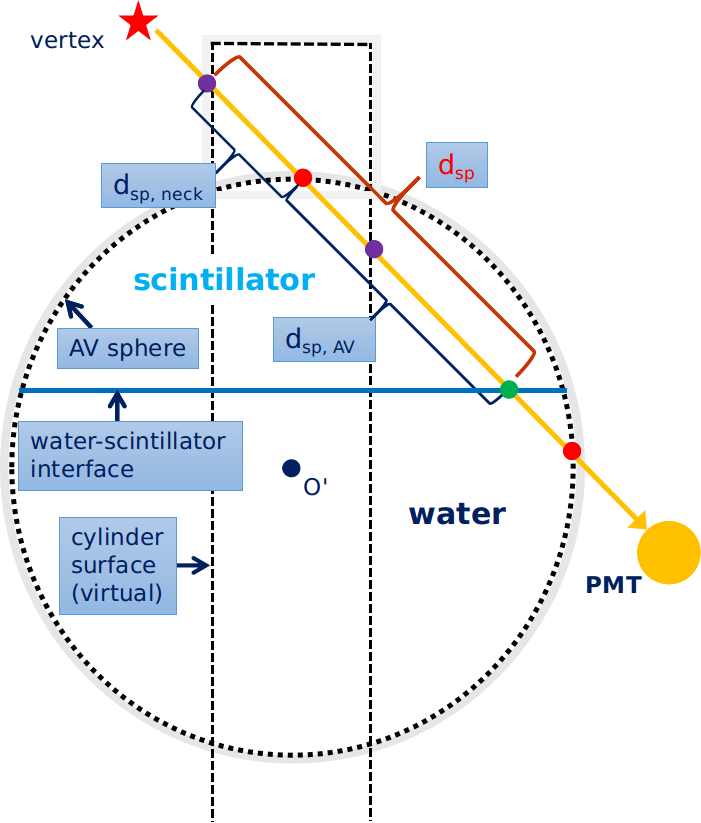
\includegraphics[width=7cm]{scintpath.png}
	\caption{Light path calculation.}
	\label{scintpath}
\end{figure}






\section{Conclusions}
 



\vspace{30mm}
\bibliographystyle{elsarticle-num}

\begin{thebibliography}{00}
\bibitem{cowanexpintro} Anderson, E.C. The Reines-Cowan Experiments. 

\url{http://permalink.lanl.gov/object/tr?what=info:lanl-repo/lareport/LA-UR-97-2534-02}
\bibitem{bethe1} H. Bethe and R. Peierls. The `neutrino'. Nature, 133:5321934.
\bibitem{bethe2} Bethe, Hans Albrecht. ``Energy production in stars." Physical Review 55.5 (1939): 434.
\bibitem{bahcall1} Bahcall, John N. ``Solar neutrinos. i. theoretical." Physical Review Letters 12.11 (1964): 300.
\bibitem{raymond} Davis Jr, Raymond. ``Solar neutrinos. ii. experimental." Physical Review Letters 12.11 (1964): 303.
\bibitem{GALLEX} Anselmann, P., et al. ``GALLEX solar neutrino observations. The results from GALLEX I and early results from GALLEX II." Physics Letters B 314.3-4 (1993): 445-458.
\bibitem{SAGE} Abdurashitov, J. N., et al. "Results from SAGE (The Russian-American gallium solar neutrino experiment)." Physics Letters B 328.1-2 (1994): 234-248.
\bibitem{bahcall2} Bahcall, John N. ``Gallium solar neutrino experiments: Absorption cross sections, neutrino spectra, and predicted event rates." Physical Review C 56.6 (1997): 3391.

\bibitem{pdg2017} C. Patrignani et al. (Particle Data Group), Chin. Phys. C, 40, 100001 (2016) and 2017 update.

\bibitem{imb} Becker-Szendy, R., Bratton, C.B., Casper, D., Dye, S.T., Gajewski, W., Goldhaber, M. et al. (1992) Electron- and muon-neutrino content of the atmospheric flux. Phys. Rev. D 46, 3720-3724.

\bibitem{soudan2} Allison, W.W.M., Alner, G.J., Ayres, D.S., Barrett, W.L., Bode, C., Border, P.M. et al. (Soudan-2 collaboration) (1997) Measurement of the atmospheric neutrino flavour composition in Soudan 2. Phys. Lett. B 391, 491-500.

\bibitem{atmNuReview} Takaaki Kajita, ``Atmospheric Neutrinos," Advances in High Energy Physics, vol. 2012, Article ID 504715, 24 pages, 2012. doi:10.1155/2012/504715

\bibitem{kamioII} Hirata, Kohji S., et al. ``Observation of $^8$B solar neutrinos in the Kamiokande-II detector." Physical Review Letters 63.1 (1989): 16.

\bibitem{herbertChen} Chen, Herbert H. ``Direct approach to resolve the solar-neutrino problem." Physical Review Letters 55.14 (1985): 1534.

\bibitem{SNO} Ahmad, Q. Retal, et al. ``Direct evidence for neutrino flavor transformation from neutral-current interactions in the Sudbury Neutrino Observatory." Physical review letters 89.1 (2002): 011301.

\bibitem{SNOresult} Aharmim, B., et al. "Combined analysis of all three phases of solar neutrino data from the Sudbury Neutrino Observatory." Physical Review C 88.2 (2013): 025501.

\bibitem{superK} Fukuda, Y., et al. ``Evidence for oscillation of atmospheric neutrinos." Physical Review Letters 81.8 (1998): 1562.

\bibitem{nobeldoc} ``The Nobel Prize in Physics 2015". Nobelprize.org. Nobel Media AB 2014. Web. 1 Oct 2017. \url{http://www.nobelprize.org/nobel_prizes/physics/laureates/2015/}

\bibitem{kamland} Eguchi, K., et al. "First results from KamLAND: evidence for reactor antineutrino disappearance." Physical Review Letters 90.2 (2003): 021802.

\bibitem{kamland_measure} Abe, S., et al. "Precision measurement of neutrino oscillation parameters with KamLAND." Physical Review Letters 100.22 (2008): 221803.


\bibitem{dayabayresults} An, Feng Peng, et al. "Measurement of electron antineutrino oscillation based on 1230 days of operation of the Daya Bay experiment." Physical Review D 95.7 (2017): 072006.

\bibitem{reactorNu} Qian, Xin, and Jen-Chieh Peng. "Physics with Reactor Neutrinos." arXiv preprint arXiv:1801.05386 (2018).


\bibitem{joseTextbook} Valle, José Wagner Furtado, and Jorge Romao. Neutrinos in high energy and astroparticle physics. John Wiley \& Sons, 2015.




\bibitem{Qian} Qian, X., \& Vogel, P. (2015). Neutrino mass hierarchy. Progress in Particle and Nuclear Physics, 83, 1-30.



\bibitem{BahcallRoadMap} Bahcall, John N., and Carlos Pena-Garay. ``A road map to solar neutrino fluxes, neutrino oscillation parameters, and tests for new physics." Journal of High Energy Physics 2003.11 (2003): 004.






\bibitem{Dai} Dai, Xiongxin, et al. ``Wavelength shifters for water Cherenkov detectors." Nuclear Instruments and Methods in Physics Research Section A: Accelerators, Spectrometers, Detectors and Associated Equipment 589.2 (2008): 290-295.

\bibitem{Brice} Stephen John Brice. Monte Carlo and Analysis Techniques for the Sudbury Neutrino Observatory. PhD thesis, Balliol College, Oxford University, 1996.


\bibitem{feynmanLatex}J. Ellis, ``TikZ-Feynman: Feynman diagrams with TikZ", (2016), arXiv:1601.05437 [hep-ph]


\bibitem{gerda} Agostini, M., et al. ``Search of Neutrinoless Double Beta Decay with the GERDA Experiment." Nuclear and Particle Physics Proceedings 273 (2016): 1876-1882. 

\bibitem{gerda2} Agostini, M., et al. ``Background-free search for neutrinoless double-$\beta$ decay of 76 Ge with GERDA." Nature 544.7648 (2017): 47.

\bibitem{exo} Albert, J. B., et al. "Search for Majorana neutrinos with the first two years of EXO-200 data." Nature 510.7504 (2014): 229.

\bibitem{nEXO} Albert, J. B., et al. ``Sensitivity and Discovery Potential of nEXO to Neutrinoless Double Beta Decay." arXiv preprint arXiv:1710.05075 (2017).


\bibitem{kamlandZen} Gando, A., et al. ``Search for Majorana neutrinos near the inverted mass hierarchy region with KamLAND-Zen." Physical review letters 117.8 (2016): 082503.

\bibitem{cuore} Alduino, C., et al. ``First Results from CUORE: A Search for Lepton Number Violation via $0\nu\beta\beta$ Decay of $^{130}$Te." arXiv preprint arXiv:1710.07988 (2017).



\bibitem{whitepaper} Andringa, S., et al. ``Current Status and Future Prospects of the SNO+." Advances in High Energy Physics 2016 (2016).

\bibitem{boulay} Boulay, Mark Guy. Direct evidence for weak flavour mixing with the Sudbury Neutrino Observatory. 2001.



\end{thebibliography}


\end{document}

%%
%% End of file `elsarticle-template-num.tex'.
